% Options for packages loaded elsewhere
\PassOptionsToPackage{unicode}{hyperref}
\PassOptionsToPackage{hyphens}{url}
\documentclass[
]{article}
\usepackage{xcolor}
\usepackage[margin=1in]{geometry}
\usepackage{amsmath,amssymb}
\setcounter{secnumdepth}{5}
\usepackage{iftex}
\ifPDFTeX
  \usepackage[T1]{fontenc}
  \usepackage[utf8]{inputenc}
  \usepackage{textcomp} % provide euro and other symbols
\else % if luatex or xetex
  \usepackage{unicode-math} % this also loads fontspec
  \defaultfontfeatures{Scale=MatchLowercase}
  \defaultfontfeatures[\rmfamily]{Ligatures=TeX,Scale=1}
\fi
\usepackage{lmodern}
\ifPDFTeX\else
  % xetex/luatex font selection
\fi
% Use upquote if available, for straight quotes in verbatim environments
\IfFileExists{upquote.sty}{\usepackage{upquote}}{}
\IfFileExists{microtype.sty}{% use microtype if available
  \usepackage[]{microtype}
  \UseMicrotypeSet[protrusion]{basicmath} % disable protrusion for tt fonts
}{}
\makeatletter
\@ifundefined{KOMAClassName}{% if non-KOMA class
  \IfFileExists{parskip.sty}{%
    \usepackage{parskip}
  }{% else
    \setlength{\parindent}{0pt}
    \setlength{\parskip}{6pt plus 2pt minus 1pt}}
}{% if KOMA class
  \KOMAoptions{parskip=half}}
\makeatother
\usepackage{graphicx}
\makeatletter
\newsavebox\pandoc@box
\newcommand*\pandocbounded[1]{% scales image to fit in text height/width
  \sbox\pandoc@box{#1}%
  \Gscale@div\@tempa{\textheight}{\dimexpr\ht\pandoc@box+\dp\pandoc@box\relax}%
  \Gscale@div\@tempb{\linewidth}{\wd\pandoc@box}%
  \ifdim\@tempb\p@<\@tempa\p@\let\@tempa\@tempb\fi% select the smaller of both
  \ifdim\@tempa\p@<\p@\scalebox{\@tempa}{\usebox\pandoc@box}%
  \else\usebox{\pandoc@box}%
  \fi%
}
% Set default figure placement to htbp
\def\fps@figure{htbp}
\makeatother
\setlength{\emergencystretch}{3em} % prevent overfull lines
\providecommand{\tightlist}{%
  \setlength{\itemsep}{0pt}\setlength{\parskip}{0pt}}
\usepackage{booktabs}
\usepackage{longtable}
\usepackage{array}
\usepackage{multirow}
\usepackage{wrapfig}
\usepackage{float}
\usepackage{colortbl}
\usepackage{pdflscape}
\usepackage{tabu}
\usepackage{threeparttable}
\usepackage{threeparttablex}
\usepackage[normalem]{ulem}
\usepackage{makecell}
\usepackage{xcolor}
\usepackage{bookmark}
\IfFileExists{xurl.sty}{\usepackage{xurl}}{} % add URL line breaks if available
\urlstyle{same}
\hypersetup{
  pdftitle={MRTT Causal Analysis},
  pdfauthor={Harshit Soni (hs5666), Gabriel Nixon Raj (gr2513)},
  hidelinks,
  pdfcreator={LaTeX via pandoc}}

\title{MRTT Causal Analysis}
\author{Harshit Soni (hs5666), Gabriel Nixon Raj (gr2513)}
\date{2026-04-16}

\begin{document}
\maketitle

{
\setcounter{tocdepth}{2}
\tableofcontents
}
\section{Data Loading}\label{data-loading}

\begin{verbatim}
## Episode data: 6800 rows, 34 seeds, 100 episodes/seed/world
\end{verbatim}

\begin{verbatim}
## Round data: 1360000 rows from 68 runs
\end{verbatim}

\section{Analysis 1: Episode-Level
G-Computation}\label{analysis-1-episode-level-g-computation}

\begingroup\fontsize{10}{12}\selectfont

\begin{longtable}[t]{lrrrr}
\caption{\label{tab:episode-point-estimates}Episode-level point estimates}\\
\toprule
Outcome & Naive & G-comp A (Full) & G-comp A (Lean) & G-comp B\\
\midrule
investor\_return & -4018.53 & -3811.21 & -4202.61 & -4018.53\\
fair\_1\_repay & 0.00 & -0.01 & 0.00 & 0.00\\
max\_1\_repay & 0.00 & 0.01 & 0.00 & 0.00\\
\bottomrule
\end{longtable}
\endgroup{}

\begin{verbatim}
##   ep boot [250/1000]
##   ep boot [500/1000]
##   ep boot [750/1000]
##   ep boot [1000/1000]
\end{verbatim}

\begingroup\fontsize{10}{12}\selectfont

\begin{longtable}[t]{llr>{}rrrr}
\caption{\label{tab:episode-eval}Episode-level: Bias, RMSE, 95\% CI Coverage}\\
\toprule
Outcome & Estimator & True ATE & Bias & RMSE & Coverage & SE\\
\midrule
Investor Return & naive & -4018.5288 & \textbf{-107.2046} & 3176.9729 & 0.954 & 3176.7524\\
Investor Return & A\_full & -4018.5288 & \textbf{1819.5630} & 12920.4363 & 0.945 & 12798.0723\\
Investor Return & A\_lean & -4018.5288 & \textbf{-354.0792} & 3312.5542 & 0.947 & 3295.2240\\
Investor Return & B & -4018.5288 & \textbf{-107.2046} & 3176.9729 & 0.954 & 3176.7524\\
Fair Repay & naive & -0.0030 & \textbf{0.0000} & 0.0045 & 0.953 & 0.0045\\
\addlinespace
Fair Repay & A\_full & -0.0030 & \textbf{-0.0052} & 0.0239 & 0.954 & 0.0233\\
Fair Repay & A\_lean & -0.0030 & \textbf{-0.0003} & 0.0047 & 0.949 & 0.0047\\
Fair Repay & B & -0.0030 & \textbf{0.0000} & 0.0045 & 0.953 & 0.0045\\
Max Repay & naive & 0.0022 & \textbf{-0.0001} & 0.0046 & 0.951 & 0.0046\\
Max Repay & A\_full & 0.0022 & \textbf{0.0107} & 0.0242 & 0.945 & 0.0218\\
\addlinespace
Max Repay & A\_lean & 0.0022 & \textbf{-0.0008} & 0.0052 & 0.941 & 0.0051\\
Max Repay & B & 0.0022 & \textbf{-0.0001} & 0.0046 & 0.951 & 0.0046\\
\bottomrule
\end{longtable}
\endgroup{}

\begin{figure}

{\centering 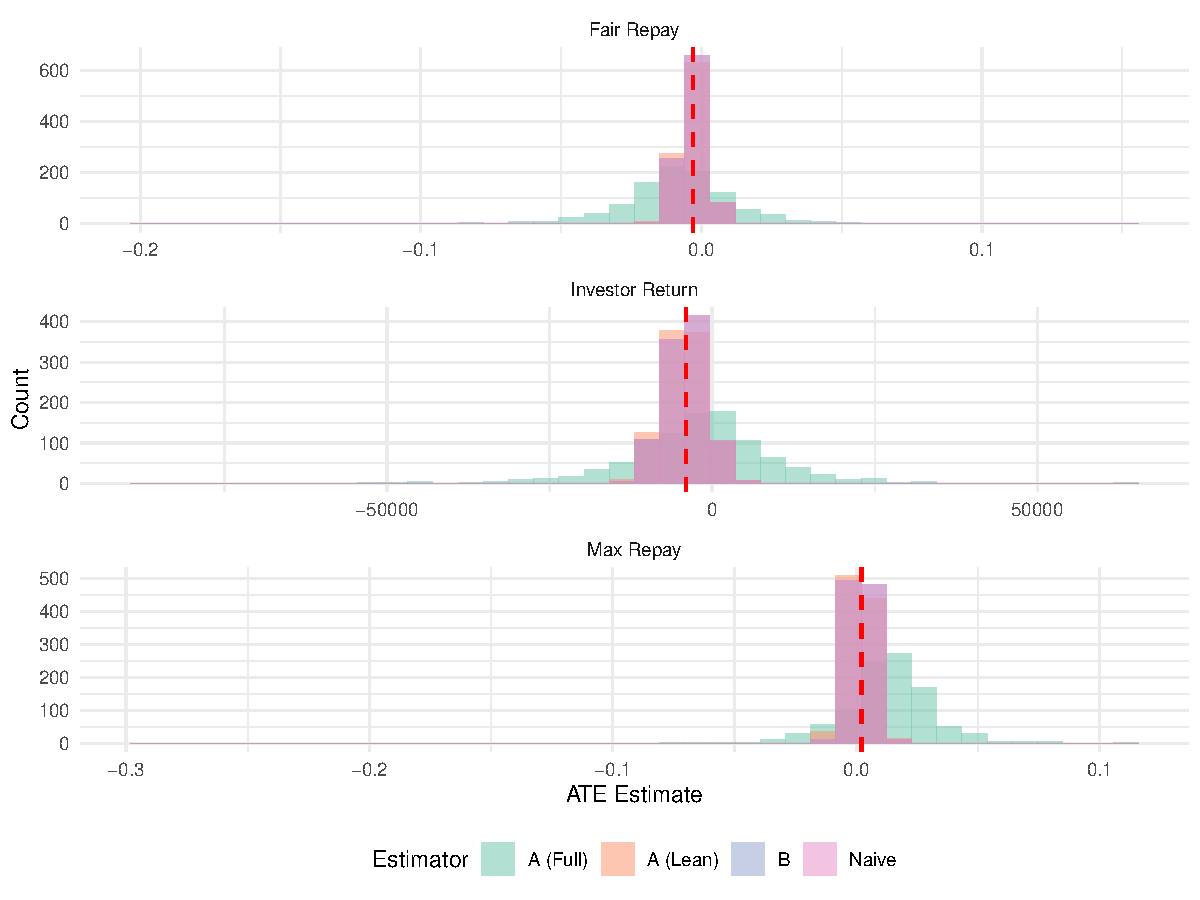
\includegraphics{causal_analysis_bare_files/figure-latex/fig-ep-bootstrap-1} 

}

\caption{Episode-level bootstrap distributions}\label{fig:fig-ep-bootstrap}
\end{figure}

\begin{figure}

{\centering 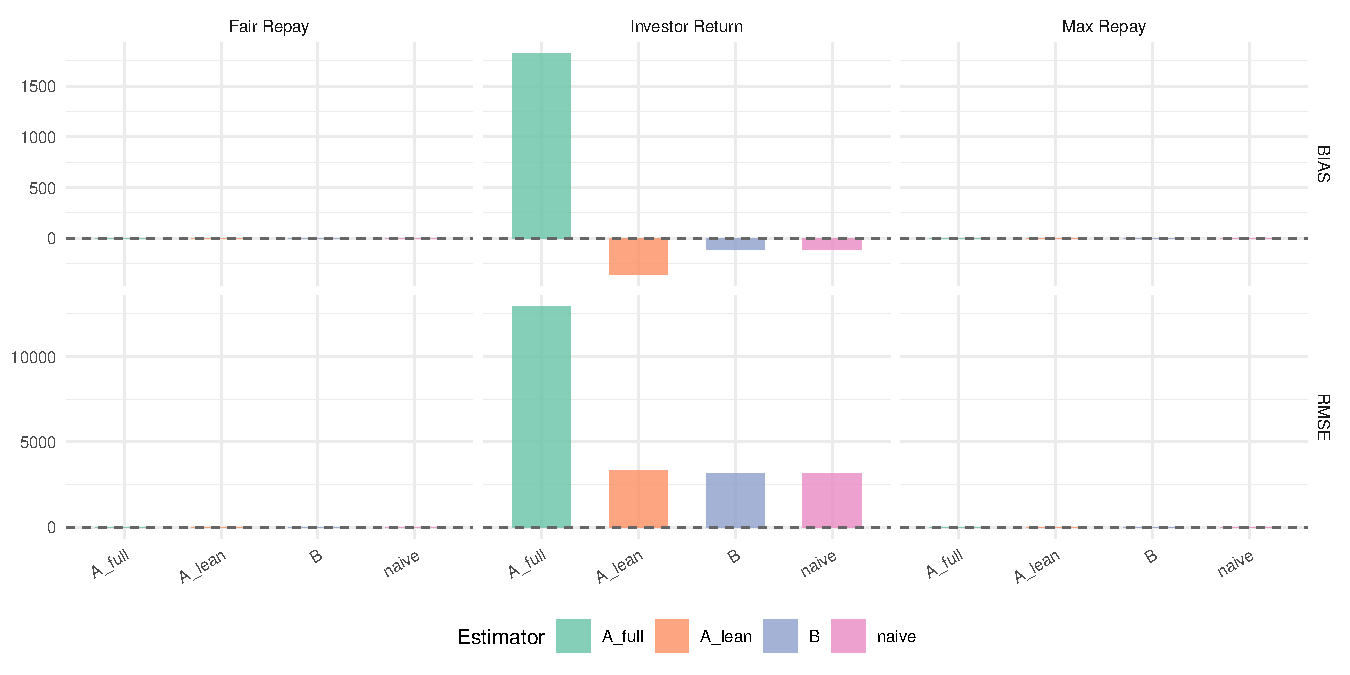
\includegraphics{causal_analysis_bare_files/figure-latex/fig-ep-metrics-1} 

}

\caption{Episode-level bias and RMSE}\label{fig:fig-ep-metrics}
\end{figure}

\begin{figure}

{\centering 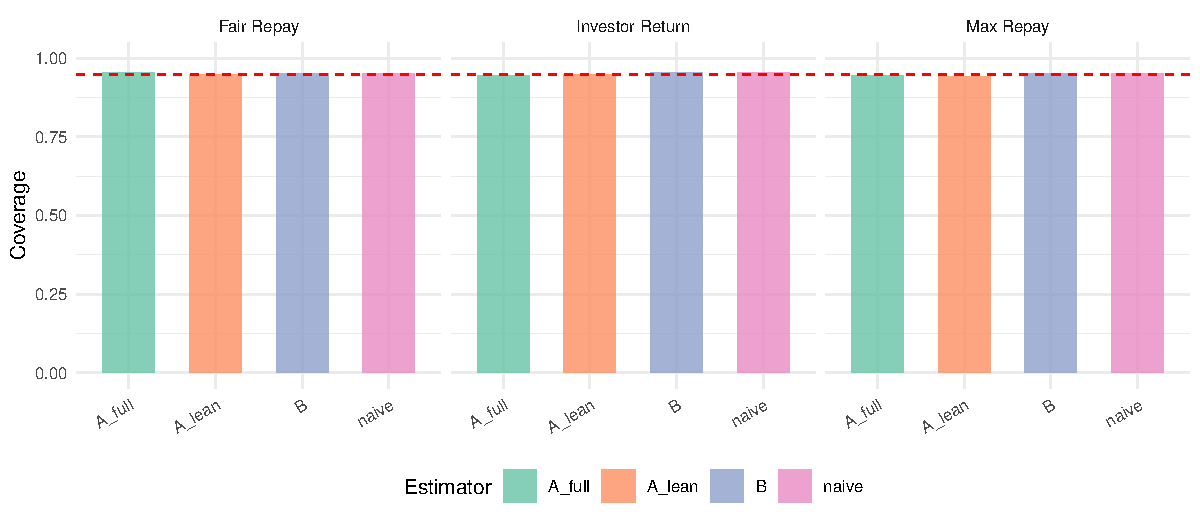
\includegraphics{causal_analysis_bare_files/figure-latex/fig-ep-coverage-1} 

}

\caption{Episode-level 95\% CI coverage}\label{fig:fig-ep-coverage}
\end{figure}

\begin{figure}

{\centering 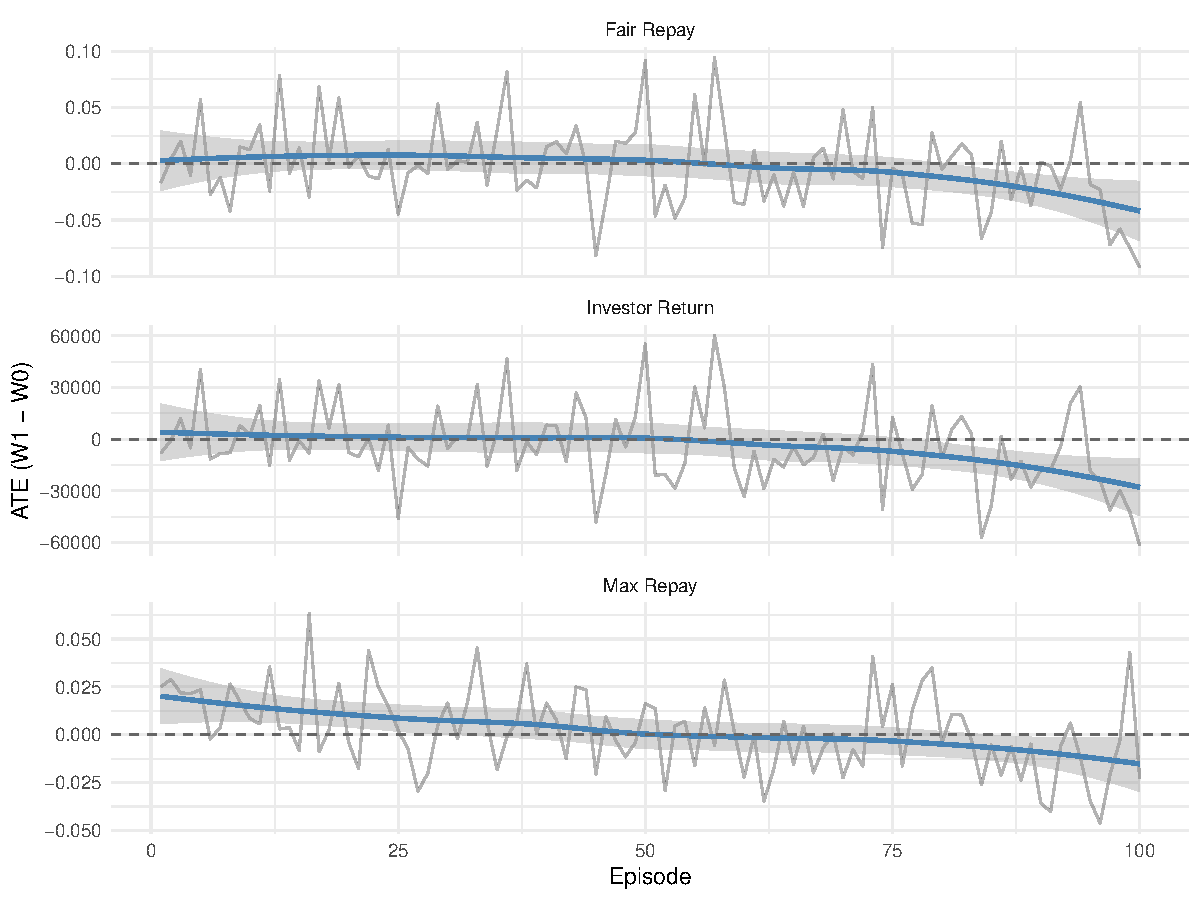
\includegraphics{causal_analysis_bare_files/figure-latex/fig-ate-episode-1} 

}

\caption{ATE by training episode}\label{fig:fig-ate-episode}
\end{figure}

\begin{figure}

{\centering 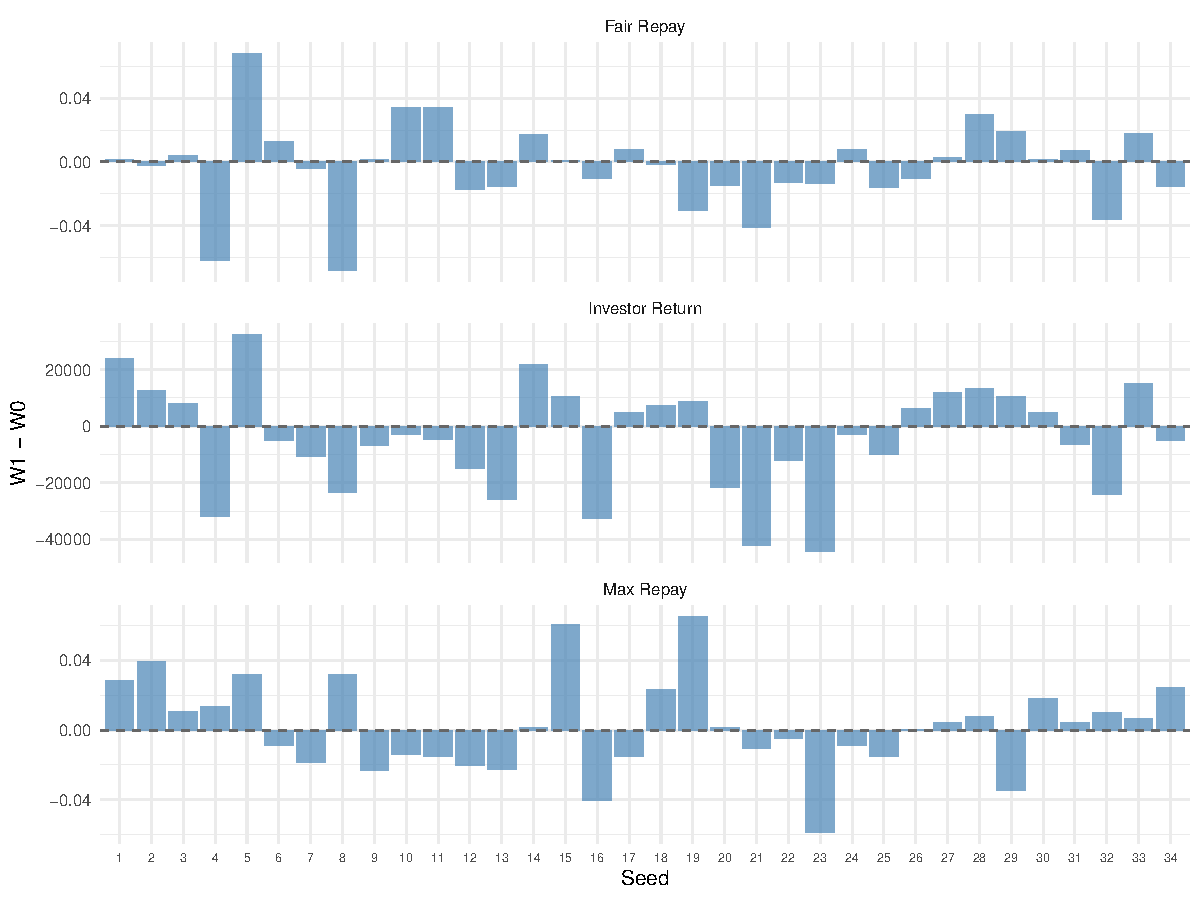
\includegraphics{causal_analysis_bare_files/figure-latex/fig-paired-1} 

}

\caption{Within-seed paired differences}\label{fig:fig-paired}
\end{figure}

\section{Analysis 2: Round-Level
G-Computation}\label{analysis-2-round-level-g-computation}

\begin{verbatim}
## Round data (subsampled): 27200 rows, h_cols found: 5
\end{verbatim}

\begin{longtable}[t]{lr}
\caption{\label{tab:round-ground-truth}Round-level ground truth ATEs}\\
\toprule
Outcome & True ATE\\
\midrule
repayment\_pct & -0.0013\\
investor\_reward & 0.4006\\
\bottomrule
\end{longtable}

\begin{verbatim}
##   rd boot [250/1000]
##   rd boot [500/1000]
##   rd boot [750/1000]
##   rd boot [1000/1000]
\end{verbatim}

\begingroup\fontsize{10}{12}\selectfont

\begin{longtable}[t]{llr>{}rrrr}
\caption{\label{tab:round-eval}Round-level: Bias, RMSE, 95\% CI Coverage}\\
\toprule
Outcome & Estimator & True ATE & Bias & RMSE & Coverage & SE\\
\midrule
Repayment \% & naive & -0.0013 & \textbf{0.0000} & 0.0226 & 0.951 & 0.0226\\
Repayment \% & A & -0.0013 & \textbf{0.0175} & 0.0226 & 0.792 & 0.0144\\
Repayment \% & B & -0.0013 & \textbf{0.0079} & 0.0200 & 0.931 & 0.0184\\
Investor Reward & naive & 0.4006 & \textbf{0.0136} & 1.2443 & 0.942 & 1.2448\\
Investor Reward & A & 0.4006 & \textbf{0.9222} & 1.2561 & 0.822 & 0.8532\\
\addlinespace
Investor Reward & B & 0.4006 & \textbf{0.6529} & 1.1762 & 0.905 & 0.9789\\
\bottomrule
\end{longtable}
\endgroup{}

\begin{figure}

{\centering 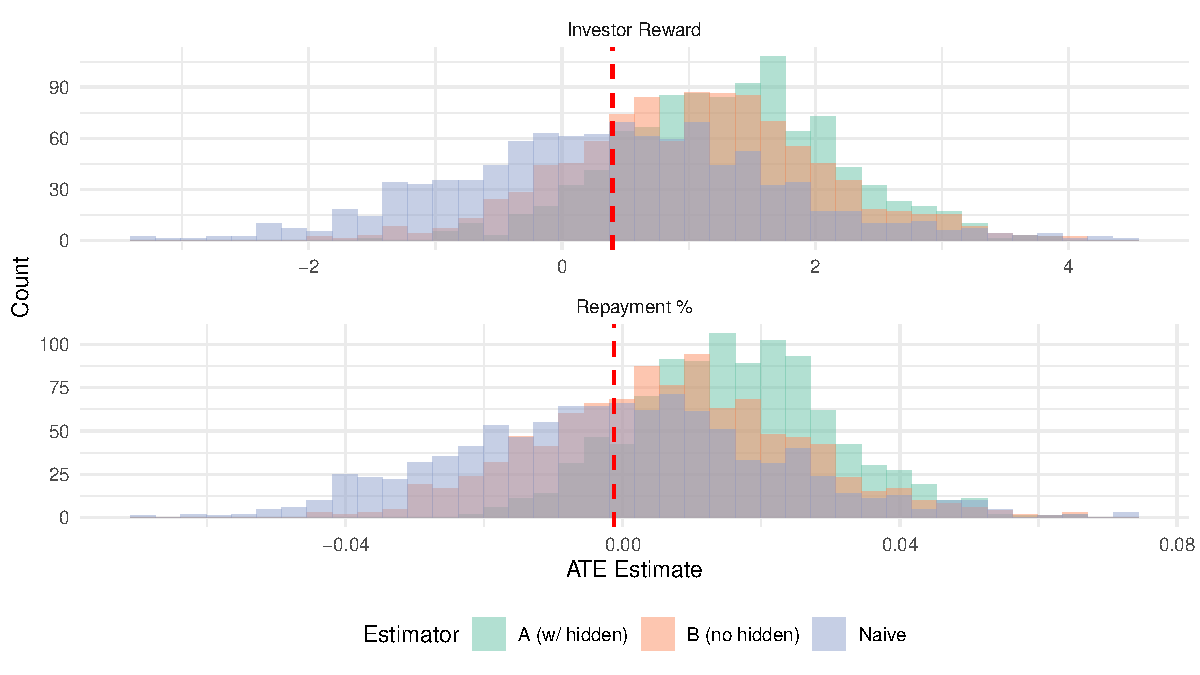
\includegraphics{causal_analysis_bare_files/figure-latex/fig-rd-bootstrap-1} 

}

\caption{Round-level bootstrap distributions}\label{fig:fig-rd-bootstrap}
\end{figure}

\begin{figure}

{\centering 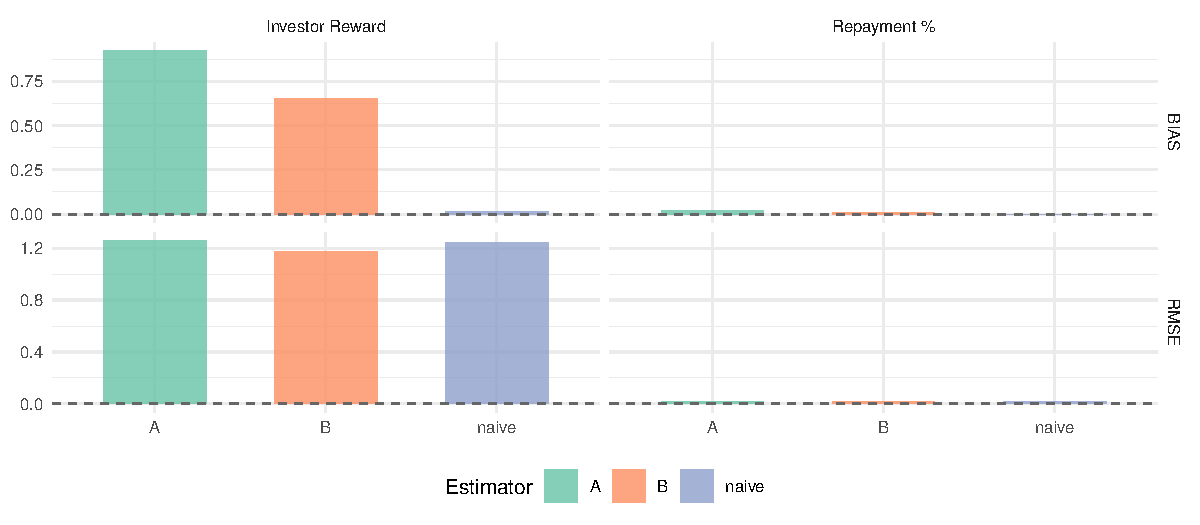
\includegraphics{causal_analysis_bare_files/figure-latex/fig-rd-metrics-1} 

}

\caption{Round-level bias and RMSE}\label{fig:fig-rd-metrics}
\end{figure}

\section{Combined Summary}\label{combined-summary}

\begingroup\fontsize{9}{11}\selectfont

\begin{longtable}[t]{lllr>{}rrrr}
\caption{\label{tab:combined-table}Combined evaluation across both analysis levels}\\
\toprule
Level & Outcome & Estimator & True ATE & Bias & RMSE & Coverage & SE\\
\midrule
Episode & Investor Return & ep\_naive & -4018.5288 & \textbf{-107.2046} & 3176.9729 & 0.954 & 3176.7524\\
Episode & Investor Return & ep\_A\_full & -4018.5288 & \textbf{1819.5630} & 12920.4363 & 0.945 & 12798.0723\\
Episode & Investor Return & ep\_A\_lean & -4018.5288 & \textbf{-354.0792} & 3312.5542 & 0.947 & 3295.2240\\
Episode & Investor Return & ep\_B & -4018.5288 & \textbf{-107.2046} & 3176.9729 & 0.954 & 3176.7524\\
Episode & Fair Repay & ep\_naive & -0.0030 & \textbf{0.0000} & 0.0045 & 0.953 & 0.0045\\
\addlinespace
Episode & Fair Repay & ep\_A\_full & -0.0030 & \textbf{-0.0052} & 0.0239 & 0.954 & 0.0233\\
Episode & Fair Repay & ep\_A\_lean & -0.0030 & \textbf{-0.0003} & 0.0047 & 0.949 & 0.0047\\
Episode & Fair Repay & ep\_B & -0.0030 & \textbf{0.0000} & 0.0045 & 0.953 & 0.0045\\
Episode & Max Repay & ep\_naive & 0.0022 & \textbf{-0.0001} & 0.0046 & 0.951 & 0.0046\\
Episode & Max Repay & ep\_A\_full & 0.0022 & \textbf{0.0107} & 0.0242 & 0.945 & 0.0218\\
\addlinespace
Episode & Max Repay & ep\_A\_lean & 0.0022 & \textbf{-0.0008} & 0.0052 & 0.941 & 0.0051\\
Episode & Max Repay & ep\_B & 0.0022 & \textbf{-0.0001} & 0.0046 & 0.951 & 0.0046\\
Round & Repayment \% & rd\_naive & -0.0013 & \textbf{0.0000} & 0.0226 & 0.951 & 0.0226\\
Round & Repayment \% & rd\_A & -0.0013 & \textbf{0.0175} & 0.0226 & 0.792 & 0.0144\\
Round & Repayment \% & rd\_B & -0.0013 & \textbf{0.0079} & 0.0200 & 0.931 & 0.0184\\
\addlinespace
Round & Investor Reward & rd\_naive & 0.4006 & \textbf{0.0136} & 1.2443 & 0.942 & 1.2448\\
Round & Investor Reward & rd\_A & 0.4006 & \textbf{0.9222} & 1.2561 & 0.822 & 0.8532\\
Round & Investor Reward & rd\_B & 0.4006 & \textbf{0.6529} & 1.1762 & 0.905 & 0.9789\\
\bottomrule
\end{longtable}
\endgroup{}

\end{document}
